\documentclass[
	a4paper,
	oneside,
	BCOR = 10mm,
	DIV = 12,
	12pt,
	headings = normal,
	%draft,
]{scrartcl}

%%% Length calculations
\usepackage{calc}
%%%

%%% Support for color
\usepackage{xcolor}
\definecolor{lightblue}{HTML}{03A9F4}
\definecolor{red}{HTML}{F44336}
%%%

%%% Including graphics
\usepackage{graphicx}
%%%

%%% Font selection
\usepackage{fontspec}

\setromanfont{STIX Two Text}[
	SmallCapsFeatures = {LetterSpace = 8},
]

\setsansfont{IBM Plex Sans}[
	Scale = MatchUppercase,
]

\setmonofont{IBM Plex Mono}[
	Scale = MatchUppercase,
]
%%%

%%% Math typesetting
\usepackage{amsmath}
\usepackage{mathtools}

\usepackage{unicode-math}
\setmathfont{STIX Two Math}

\usepackage{IEEEtrantools}
%%%

%%% List settings
\usepackage{enumitem}
\setlist[enumerate]{%
	label*      = {\arabic*.},
	left        = \parindent,
	topsep      = 0\baselineskip,
	parsep      = 0\baselineskip,
	itemsep     = 0\baselineskip,
	noitemsep, % override itemsep
}

\setlist[itemize]{%
	label       = {—},
	left        = \parindent,
	topsep      = 0\baselineskip,
	parsep      = 0\baselineskip,
	itemsep     = 0\baselineskip,
	noitemsep, % override itemsep
}

\setlist[description]{%
	font        = {\rmfamily\upshape\bfseries},
	topsep      = 1\baselineskip,
	parsep      = 0\baselineskip,
	itemsep     = 0\baselineskip,
}

% Manual bibliography list
\newlist{manualbib}{enumerate}{1}
\setlist[manualbib]{%
	label      = {\arabic*.},
	leftmargin = 0em, 
	topsep      = 0\baselineskip,
	parsep      = 0\baselineskip,
	itemsep     = 0\baselineskip,
	noitemsep, % override itemsep
}

%%%

%%% Structural elements typesetting
\setkomafont{pagenumber}{\rmfamily\upshape}
\setkomafont{disposition}{\rmfamily\bfseries}

% Sectioning
\RedeclareSectionCommand[
	beforeskip = -1\baselineskip,
	afterskip  = 1\baselineskip,
	font       = {\normalsize\bfseries\scshape},
]{section}

%% Start new sections from a new page
\usepackage{etoolbox}
\preto\section{\clearpage}

\RedeclareSectionCommand[
	beforeskip = -1\baselineskip,
	afterskip  = 1\baselineskip,
	font       = {\normalsize\bfseries\itshape},
]{subsection}

\RedeclareSectionCommand[
	beforeskip = -1\baselineskip,
	afterskip  = 1\baselineskip,
	font       = {\normalsize\bfseries},
]{subsubsection}

\RedeclareSectionCommand[
	beforeskip = -1\baselineskip,
	afterskip  = -0.5em,
	font       = {\normalsize\mdseries\scshape\addfontfeatures{Letters = {UppercaseSmallCaps}}},
]{paragraph}
%%%

%%% Typographic enhancements
\usepackage{microtype}
%%%

%%% Language-specific settings
\usepackage{polyglossia}
\setmainlanguage{ukrainian}
\setotherlanguages{english}
%%%

%%% Captions
\usepackage{caption}
\usepackage{subcaption}

%\DeclareCaptionLabelFormat{closing}{#2)}
%\captionsetup[subtable]{labelformat = closing}

%\captionsetup[subfigure]{labelformat = closing}

\captionsetup[table]{%
	aboveskip = 0\baselineskip,
	belowskip = 0\baselineskip,
}

\captionsetup[figure]{%
	aboveskip = 1\baselineskip,
	belowskip = 0\baselineskip,
}

\captionsetup[subfigure]{%
	labelformat = simple,
	labelformat = brace,
}
%%%

%%% Hyphenated ragged typesetting
\usepackage{ragged2e}
%%%

%%% Table typesetting
\usepackage{booktabs}
\usepackage{longtable}

\usepackage{multirow}

\usepackage{array}
\newcolumntype{v}[1]{>{\RaggedRight\arraybackslash\hspace{0pt}}p{#1}}
\newcolumntype{b}[1]{>{\Centering\arraybackslash\hspace{0pt}}p{#1}}
\newcolumntype{n}[1]{>{\RaggedLeft\arraybackslash\hspace{0pt}}p{#1}}
%%%

%%% Drawing
\usepackage{tikz}
\usepackage{tikzscale}
\usetikzlibrary{arrows.meta} % Stealth arrow tips
\usetikzlibrary{calc} % Coordinate calculations
\usetikzlibrary{datavisualization}
\usetikzlibrary{plotmarks}
\usetikzlibrary{positioning}
\usetikzlibrary{shapes.geometric} % Stealth arrow tips

\usepackage{tikzscale}
%%%

%%% SI units typesetting
\usepackage{siunitx}
\sisetup{%
	output-decimal-marker = {,},
	exponent-product      = {\cdot},
	inter-unit-product    = \ensuremath{{} \cdot {}},
	per-mode              = symbol,
	round-mode            = places,
	round-precision       = 3,
}
%%%

%%% Framing code listings
\usepackage{tcolorbox}
\tcbuselibrary{breakable}
\tcbuselibrary{minted}
\tcbuselibrary{skins}

\newtcblisting[
	auto counter,
	list inside,
	number within = section,
]{listingpython}[3][]{%
	minted language = python,
	minted style    = bw,
	minted options  = {%
		linenos,
		tabsize = 4,
		breaklines,
		% breakanywhere,
		fontsize = \footnotesize,
		autogobble
	},
	%
	% empty,
	sharp corners,
	colframe         = black,
	colback          = black!0,
	leftrule         = 0em,
	rightrule        = 0em,
	toprule          = 1pt, % orig = 0pt
	bottomrule       = 1pt, % orig = 0pt
	titlerule        = 0.5pt,
	colbacktitle     = black!0,
	coltitle         = black,
	toptitle         = 0.3em,
	bottomtitle      = 0.1em,
	borderline north = {1pt}{0pt}{black},
	borderline south = {1pt}{0pt}{black},
	before skip      = \intextsep,
	after  skip      = \intextsep,
	title            = {Лістинг \thetcbcounter: #2},
	list entry       = {\protect\numberline{\thetcbcounter}#2},
	left = 0em,
	right = 0em,
	%
	listing only,
	breakable,
	%
	label = {#3},
	%
	#1
}

\newtcbinputlisting[auto counter, list inside, number within = section]{\inputpython}[4][]{%
	minted language = python,
	minted style    = bw,
	minted options  = {%
		linenos,
		tabsize = 4,
		breaklines,
		breakbytokenanywhere,
		fontsize = \footnotesize,
	},
	%
	% empty,
	sharp corners,
	colframe         = black,
	colback          = black!0,
	leftrule         = 0em,
	rightrule        = 0em,
	toprule          = 0pt, % orig = 0pt
	bottomrule       = 0pt, % orig = 0pt
	titlerule        = 0.5pt,
	colbacktitle     = black!0,
	coltitle         = black,
	toptitle         = 0.3em,
	bottomtitle      = 0.1em,
	borderline north = {1pt}{0pt}{black},
	borderline south = {1pt}{0pt}{black},
	before skip      = \intextsep,
	after  skip      = \intextsep,
	title            = {Лістинг \thetcbcounter: #3},
	list entry       = {\protect\numberline{\thetcbcounter}#3},
	left = 0em,
	right = 0em,
	%
	listing file={#2},
	listing only,
	breakable,
	%
	label = {#4},
	%
	#1
}

% Customize minted
\usepackage{minted}
\setmintedinline{%
	style = bw,
	breaklines,
}

% Customize minted line numbers
\renewcommand{\theFancyVerbLine}{\ttfamily\scriptsize\arabic{FancyVerbLine}}

%%%

%%% Sideways table
\usepackage{pdflscape}
%%%

%%% Wrap text after sideways table
\usepackage{afterpage}
%%%

%%% Links and hyperreferences
\usepackage{hyperref}
\hypersetup{%
	bookmarksnumbered = true,
	colorlinks      = false,
	linkbordercolor = red,
	urlbordercolor  = lightblue,
	pdfborderstyle  = {/S/U/W 1.5},
}
%%%

%%% Length adjustments
% Set baselineskip, default is 14.5 pt
\linespread{1.068966} % ~15.5 pt
\setlength{\emergencystretch}{1em}
\setlength{\parindent}{1.5em}
\newlength{\gridunitwidth}
\setlength{\gridunitwidth}{\textwidth / 12}
%%%

%%% Custom commands
\newcommand{\allcaps}[1]{{\addfontfeatures{LetterSpace = 8, Kerning = Off}#1}}
\newcommand{\filename}[1]{\texttt{#1}}
\newcommand{\progname}[1]{\texttt{#1}}
\newcommand{\modulename}[1]{\texttt{#1}}
%%%

%%% Custom math commands
\newcommand{\longvar}[1]{\mathit{#1}}
\DeclarePairedDelimiter{\ceil}{\lceil}{\rceil}
%%%

\begin{document}

\begin{titlepage}
		\begin{center}
			Міністерство освіти і~науки України\\
			Національний авіаційний університет\\
			Навчально-науковий інститут комп'\-ютерних інформаційних технологій\\
			Кафедра комп'\-ютеризованих систем управління

			\vspace{\fill}
				Курсовий проект\\
				з~дисципліни «Комп'\-ютерні системи»\\
				Варіант~№~8

			\vspace{\fill}

			\begin{flushright}
				Виконав:\\
				студент \allcaps{ННІКІТ}\\
				групи СП-325\\
				Клокун В.\,Д.\\
				Перевірив:\\
				Жуков І.\,А.
			\end{flushright}

			Київ 2019
		\end{center}
	\end{titlepage}

	\tableofcontents
	\clearpage

	\section{Завдання}
		Варіант завдання на~курсовий проект визначався за~списком групи, тому необхідно виконати варіант №~8, в~якому необхідно дослідити топологічні характеристики паралельних обчислювальних систем з~масивно-паралельними архітектурами за~заданим кластером~(рис.~\ref{fig:task-cluster}).

		\begin{figure}[!htbp]
			\centering
			\includegraphics[height=8\baselineskip]{./assets/cluster-08-00-raw.pdf}
			\caption{Граф заданого кластера}
			\label{fig:task-cluster}
		\end{figure}

	\section{Теоретичні відомості}
		Метою курсової роботи є~дослідження основних топологічних характеристик паралельних обчислювальних систем з~масивно-паралельними архітектурами (\textenglish{massive parallel processing}, \textenglish{MPP}-системи).

		\textenglish{MPP}-системи~— це~багатопроцесорні системи з~розподіленою (локальною) оперативною пам'яттю. Їхня основна перевага~— необмежена масштабованість (можливість збільшення кількості процесорів у~системі без зміни її~властивостей). У~зв'язку із~цим \textenglish{MPP}-систем містять сотні, тисячі процесорів. Так, у~цей час, найбільш продуктивні \textenglish{MPP}-системи у~світі містять близько мільйона процесорів. Відомо два способи взаємозв'язків між процесорами в~\textenglish{MPP}-системі:
		\begin{itemize}
			\item статичний, коли процесори зв'язані за~допомогою спеціальних двунаправлених каналів;
			\item динамічний, коли для взаємозв'язків між процесорами використовують комутатори.
		\end{itemize}
		У~першому випадку процесори в~\textenglish{MPP}-системах можуть поєднуватися в~різні топології, а~в~другому випадку~— являють собою тільки повнозв’язану топологію.

		\begin{figure}[!htbp]
			\centering
			\includegraphics[height = 12\baselineskip]{./assets/y03s02-compsys-coursework-01-p00-mpp-topology-types.jpg}
			\caption{Приклади топологій \textenglish{MPP}-систем: а)~— повнозв'язана система, б)~— зірка, в)~— кільце, г)~— лінійка, д)~— дерево, є)~— гіперкуб 3-го~порядку, ж)~— решітка, з)~— тор}
			\label{fig:mpp-topology-types}
		\end{figure}

		У~даній роботі розглядається \textenglish{MPP}-системи зі~статичними взаємозв'язками. Для таких систем існує множина топологічних характеристик. Основними топологічними характеристиками є: 
		\begin{enumerate}
			\item Діаметр системи ($D$)~— це~мінімальна відстань між двома максимально віддаленими процесорами. Наприклад, діаметр для повнозв’язаної системи дорівнює~1, а~для топології «зірка» дорівнює~2. Діаметр кільцевої топології дорівнює~$n/2$, а~лінійної топології дорівнює~$(n - 1)$, де~$n$~— кількість процесорів у~системі. Оптимальним є~мінімальне значення діаметра. Приклади різних графів топологій систем наведені на~рис.~\ref{fig:mpp-topology-types}.
			\item Середній діаметр ($\overline{D}$). Ця~характеристика визначається за~формулою:
				\begin{IEEEeqnarray}{rCl}
					\overline{D} = \frac{
						\sum\limits_{i=1}^{n}
						\sum\limits_{j=1}^{n-1}
						d_{ij}
					}{
						n(n-1)
					}
				\end{IEEEeqnarray}
				де~$d_{ij}$~— мінімальна відстань між $i$-м~та~$j$-м~процесорами. Оптимальним є~мінімальне значення середнього діаметра.
			\item Степінь ($S$). Ця~характеристика визначається як~максимальна кількість дуг (зв'язків), інцидентні вершині (процесору) у~графі топології системи. Так, степінь лінійної й~кільцевої топології дорівнює~2, повнозв’язної топології дорівнює~$(n - 1)$.
			\item Вартість ($C$). Існує множина варіантів визначення вартості системи. Відповідно до~одного з~них вартість визначається як~сумарна кількість зв'язків у~системі. Відповідно до~іншого варіанта вартість визначається за~формулою:
				\begin{IEEEeqnarray}{rCl}
					C = D n S.
				\end{IEEEeqnarray}
				У~роботі можна використати будь-який варіант визначення вартості. Оптимальним є~мінімальне значення вартості.
			\item Топологічний трафік ($T$).	Ця~характеристика визначається за~формулою:
				\begin{IEEEeqnarray}{rCl}
					T = \frac{2 \overline{D}}{S}.
				\end{IEEEeqnarray}
				Топологічний трафік визначає степінь використання зв'язків у~системі. Оптимальне значення $T = 1$, що~означає потенційне використання всіх наявних зв'язків між процесорами. Якщо $T < 1$, це~означає, що~частина фізичних зв'язків у~системі при пересиланні даних не~будуть використані. Якщо ж~$T > 1$, при пересиланні даних зв'язків, які є~в~системі, буде недостатньо, тобто можливі додаткові тимчасові затримки.
		\end{enumerate}

	\section{Хід виконання роботи}
		\subsection{Визначення порядку нумерації процесорів у~кластерах системи при масштабуванні}
		\label{ssec:scaling}
			Спочатку визначимо порядок нумерації процесорів у~заданому кластері. Будемо нумерувати процесори зліва-направо, зверху вниз. Визначившись з~порядком, побудуємо відповідний граф заданого кластера~(рис.~\ref{fig:cluster-08-01-named}).

			\begin{figure}[!htbp]
				\centering
				\includegraphics[height=7\baselineskip]{./assets/cluster-08-01-named.pdf}
				\caption{Граф-схема заданого кластера з~пронумерованими вершинами}
				\label{fig:cluster-08-01-named}
			\end{figure}

			Пронумерувавши кластер та~побудувавши його граф-схему, переходимо до~наступного етапу~— масштабування систем за~топологіями.

			\subsubsection{Топологія «Лінійка»}
				Як~зрозуміло з~назви, топологія «Лінійка» масштабується лінійно: кожен кластер послідовно під'єднується до~обраної вершини попереднього кластера. Промасштабуємо заданий кластер для топології «Лінійка»~(рис.~\ref{fig:cluster-08-02-line-s01}, \ref{fig:cluster-08-02-line-s02}, \ref{fig:cluster-08-02-line-s03}, \ref{fig:cluster-08-02-line-s04}).

				\begin{figure}[!htbp]
					\centering
					\includegraphics[height=7\baselineskip]{./assets/cluster-08-01-named.pdf}
					\caption{Масштабування топології «Лінійка», крок~1}
					\label{fig:cluster-08-02-line-s01}
				\end{figure}

				\begin{figure}[!htbp]
					\centering
					\includegraphics[height=7\baselineskip]{./assets/cluster-08-02-line-s02.pdf}
					\caption{Масштабування топології «Лінійка», крок~2}
					\label{fig:cluster-08-02-line-s02}
				\end{figure}

				\begin{figure}[!htbp]
					\centering
					\includegraphics[height=7\baselineskip]{./assets/cluster-08-02-line-s03.pdf}
					\caption{Масштабування топології «Лінійка», крок~3}
					\label{fig:cluster-08-02-line-s03}
				\end{figure}

				\begin{figure}[!htbp]
					\centering
					\includegraphics[width=\columnwidth]{./assets/cluster-08-02-line-s04.pdf}
					\caption{Масштабування топології «Лінійка», крок~4}
					\label{fig:cluster-08-02-line-s04}
				\end{figure}

				На~кроці~4~(рис.~\ref{fig:cluster-08-02-line-s04}) вже видно, за~яким принципом масштабується топологія~«Лінійка», тому завершуємо її~масштабування.

			\subsubsection{Топологія «Зірка»}
				При використанні топології «Зірка» кожен новий кластер під'\-є\-дну\-є\-ться до~обраної вершини центрального кластера. Виконаємо масштабування заданого кластера для топології «Зірка»~(рис.~\ref{fig:cluster-08-03-star-s01}, \ref{fig:cluster-08-03-star-s02}, \ref{fig:cluster-08-03-star-s03}, \ref{fig:cluster-08-03-star-s04}).

				\begin{figure}[!htbp]
					\centering
					\includegraphics[height=5\baselineskip]{./assets/cluster-08-01-named.pdf}
					\caption{Масштабування топології «Зірка», крок~1}
					\label{fig:cluster-08-03-star-s01}
				\end{figure}

				\begin{figure}[!htbp]
					\centering
					\includegraphics[height=10\baselineskip]{./assets/cluster-08-03-star-s02.pdf}
					\caption{Масштабування топології «Зірка», крок~2}
					\label{fig:cluster-08-03-star-s02}
				\end{figure}

				\begin{figure}[!htbp]
					\centering
					\includegraphics[height=10\baselineskip]{./assets/cluster-08-03-star-s03.pdf}
					\caption{Масштабування топології «Зірка», крок~3}
					\label{fig:cluster-08-03-star-s03}
				\end{figure}

				\begin{figure}[!htbp]
					\centering
					\includegraphics[height=15\baselineskip]{./assets/cluster-08-03-star-s04.pdf}
					\caption{Масштабування топології «Зірка», крок~4}
					\label{fig:cluster-08-03-star-s04}
				\end{figure}

				\begin{figure}[!htbp]
					\centering
					\includegraphics[height=15\baselineskip]{./assets/cluster-08-03-star-s05.pdf}
					\caption{Масштабування топології «Зірка», крок~5}
					\label{fig:cluster-08-03-star-s05}
				\end{figure}

				На~кроці~5~(рис.~\ref{fig:cluster-08-03-star-s05}) вже наочно видно, за~яким принципом масштабується топологія~«Зірка», тому завершуємо її~масштабування.

			\subsubsection{Топологія «Кільце»}
				При використанні топології «Кільце» кожен новий кластер з'єднується з~обраною вершиною попереднього кластера, а~також останній~— з~першим, щоб замкнути кільце. Виконаємо масштабування заданого кластера для топології «Кільце»~(рис.~\ref{fig:cluster-08-04-ring-s01}, \ref{fig:cluster-08-04-ring-s02}, \ref{fig:cluster-08-04-ring-s03}, \ref{fig:cluster-08-04-ring-s04}, \ref{fig:cluster-08-04-ring-s05}).

				\begin{figure}[!htbp]
					\centering
					\includegraphics[height=6\baselineskip]{./assets/cluster-08-01-named.pdf}
					\caption{Масштабування топології «Кільце», крок~1}
					\label{fig:cluster-08-04-ring-s01}
				\end{figure}

				\begin{figure}[!htbp]
					\centering
					\includegraphics[height=6\baselineskip]{./assets/cluster-08-04-ring-s02.pdf}
					\caption{Масштабування топології «Кільце», крок~2}
					\label{fig:cluster-08-04-ring-s02}
				\end{figure}

				\begin{figure}[!htbp]
					\centering
					\includegraphics[height=6\baselineskip]{./assets/cluster-08-04-ring-s03.pdf}
					\caption{Масштабування топології «Кільце», крок~3}
					\label{fig:cluster-08-04-ring-s03}
				\end{figure}

				\begin{figure}[!htbp]
					\centering
					\includegraphics[width=\columnwidth]{./assets/cluster-08-04-ring-s04.pdf}
					\caption{Масштабування топології «Кільце», крок~4}
					\label{fig:cluster-08-04-ring-s04}
				\end{figure}

				\begin{figure}[!htbp]
					\centering
					\includegraphics[width=\columnwidth]{./assets/cluster-08-04-ring-s05.pdf}
					\caption{Масштабування топології «Кільце», крок~5}
					\label{fig:cluster-08-04-ring-s05}
				\end{figure}

				На~кроці~5~(рис.~\ref{fig:cluster-08-04-ring-s05}) вже наочно видно, за~яким принципом масштабується топологія~«Кільце», тому завершуємо її~масштабування.

			\subsubsection{Топологія «Решітка»}
				При використанні топології «Решітка» кожен новий кластер під'єднується до~обраної вершини своїх двох найближчих сусідів зліва та~згори. Нарощування решітки відбувається так: поки решітка не~квадратна, і~поточний рядок не~заповнений, додаємо кластер до~поточного рядка. Якщо рядок заповнений, переходимо на~новий і~повторюємо вищеописані кроки; якщо решітка квадратна~— додаємо новий кластер у~перший рядок по~горизонталі. Виконаємо масштабування заданого кластера для топології «Решітка»~(рис.~\ref{fig:cluster-08-05-grid-s01}, \ref{fig:cluster-08-05-grid-s02}, \ref{fig:cluster-08-05-grid-s03}, \ref{fig:cluster-08-05-grid-s04}).

				\begin{figure}[!htbp]
					\centering
					\includegraphics[height=7\baselineskip]{./assets/cluster-08-01-named.pdf}
					\caption{Масштабування топології «Решітка», крок~1}
					\label{fig:cluster-08-05-grid-s01}
				\end{figure}

				\begin{figure}[!htbp]
					\centering
					\includegraphics[height=6\baselineskip]{./assets/cluster-08-05-grid-s02.pdf}
					\caption{Масштабування топології «Решітка», крок~2}
					\label{fig:cluster-08-05-grid-s02}
				\end{figure}

				\begin{figure}[!htbp]
					\centering
					\includegraphics[height=12\baselineskip]{./assets/cluster-08-05-grid-s03.pdf}
					\caption{Масштабування топології «Решітка», крок~3}
					\label{fig:cluster-08-05-grid-s03}
				\end{figure}

				\begin{figure}[!htbp]
					\centering
					\includegraphics[height=12\baselineskip]{./assets/cluster-08-05-grid-s04.pdf}
					\caption{Масштабування топології «Решітка», крок~4}
					\label{fig:cluster-08-05-grid-s04}
				\end{figure}

				\begin{figure}[!htbp]
					\centering
					\includegraphics[height=12\baselineskip]{./assets/cluster-08-05-grid-s05.pdf}
					\caption{Масштабування топології «Решітка», крок~5}
					\label{fig:cluster-08-05-grid-s05}
				\end{figure}

				\begin{figure}[!htbp]
					\centering
					\includegraphics[height=12\baselineskip]{./assets/cluster-08-05-grid-s06.pdf}
					\caption{Масштабування топології «Решітка», крок~6}
					\label{fig:cluster-08-05-grid-s06}
				\end{figure}

				На~кроці~6~(рис.~\ref{fig:cluster-08-05-grid-s05}) вже наочно видно, за~яким принципом масштабується топологія~«Решітка», тому завершуємо приклад її~масштабування.

		\subsection{Визначення кількості процесорів, які додаються на~кожному кроці масштабування}
			Визначаємо кількість процесорів, які додаються на~кожному кроці масштабування. За~граф-схемою кластера з~пронумерованими процесорами видно, що~кластер містить 8~процесорів, отже, на~кожному кроці масштабування при підключені нового кластеру кількість процесорів системи збільшуватиметься на~8.

			Завдання курсового проекту передбачає, що~треба масштабувати систему, поки кількість процесорів у~системі не~стане більшою за~100. Визначимо кінцеву кількість процесорів~$n_{\text{f}}$. Нехай~$n_{\text{c}}$~— кількість процесорів у~кластері, а~$n_{\text{t}}$~— цільова кількість процесорів. Тоді кінцева кількість процесорів~$n_{\text{f}}$ обчислюється так:
			\begin{IEEEeqnarray*}{rCl}
				n_{\text{f}}
				= \ceil[\Bigg]{
						\frac{
							n_{\text{t}}
						}{
							n_{\text{c}}
						}
					}
					\cdot
					n_{\text{c}}
				= \ceil[\Bigg]{
						\frac{
							100
						}{
							8
						}
					}
					\cdot
					8
				= 13 \cdot 8 = 104,
			\end{IEEEeqnarray*}
			де~$\ceil{x}$~— функція округлення до~більшого значення.

			Отже, початкова кількість процесорів у~топології~$n_{\text{c}} = 8$, остаточна кількість після останнього кроку масштабування~$n_{\text{f}} = 104$. Визначивши кількості процесорів, що~додаються на~кожному кроці, а~також остаточну кількість процесорів, переходимо до~масштабування топологій. 

		\subsection{Опис внутрішньо- та~міжкластерних зв'язків при масштабуванні}
			При масштабуванні внутрішньокластерні зв'язки не~змінюються, оскільки при масштабуванні топологій кластери під'єднуються до~заданих процесорів, тобто створюється тільки новий міжкластерний зв'язок. Опис міжкластерних зв'язків при масштабуванні наведений відповідно для кожної топології~(пп.~\ref{ssec:scaling}).

		\subsection{Обчислення топологічних характеристик}
			Промасштабувавши топології «Лінійка», «Зірка», «Кільце» і~Решітка», обчислюємо їх~топологічні характеристики для кожного кроку масштабування. До~досліджуваних топологічних характеристик належать: діаметр~$D$, середній діаметр~$\overline{D}$, степінь~$S$, вартість~$C$ і~трафік~$T$. Заносимо отримані значення у~таблиці: для топології «Лінійка»~— табл.~\ref{tab:line-topology-characteristics}, для~топології «Зірка»~— табл.~\ref{tab:star-topology-characteristics}, для~топології «Кільце»~— табл.~\ref{tab:ring-topology-characteristics}, для~топології «Решітка»~— табл.~\ref{tab:grid-topology-characteristics}.

				\begin{table}[!htbp]
					\centering
					\caption{Залежність топологічних характеристик від кількості процесорів під час масштабування топологією «Лінійка»}
					\label{tab:line-topology-characteristics}
					\begin{tabular}{
						v{2\gridunitwidth - 2\tabcolsep}
						*{5}{n{2\gridunitwidth - 2\tabcolsep}}
					}
						\toprule
							& \multicolumn{5}{c}{Топологічні характеристики}\\
							\cmidrule(lr){2-6}
							К-кість проц.~$n$ &
							Діаметр~$D$ &
							Середній діаметр~$\overline{D}$ &
							Степінь~$S$ &
							Вартість~$C$ &
							Трафік~$T$\\
						\midrule
							\num{8} & \num{2} & \num{1,28571428571428} & \num{7} & \num{20} & \num{0,36734693877551}\\
							\num{16} & \num{3} & \num{2,06666666666666} & \num{8} & \num{41} & \num{0,516666666666666}\\
							\num{24} & \num{4} & \num{2,53623188405797} & \num{9} & \num{62} & \num{0,563607085346215}\\
							\num{32} & \num{5} & \num{2,93548387096774} & \num{9} & \num{83} & \num{0,652329749103942}\\
							\num{40} & \num{6} & \num{3,3076923076923} & \num{9} & \num{104} & \num{0,735042735042735}\\
							\num{48} & \num{7} & \num{3,66666666666666} & \num{9} & \num{125} & \num{0,814814814814814}\\
							\num{56} & \num{8} & \num{4,01818181818181} & \num{9} & \num{146} & \num{0,892929292929293}\\
							\num{64} & \num{9} & \num{4,36507936507936} & \num{9} & \num{167} & \num{0,970017636684303}\\
							\num{72} & \num{10} & \num{4,70892018779342} & \num{9} & \num{188} & \num{1,04642670839853}\\
							\num{80} & \num{11} & \num{5,0506329113924} & \num{9} & \num{209} & \num{1,12236286919831}\\
							\num{88} & \num{12} & \num{5,39080459770114} & \num{9} & \num{230} & \num{1,19795657726692}\\
							\num{96} & \num{13} & \num{5,7298245614035} & \num{9} & \num{251} & \num{1,27329434697855}\\
							\num{104} & \num{14} & \num{6,06796116504854} & \num{9} & \num{272} & \num{1,34843581445523}\\
						\bottomrule
					\end{tabular}
				\end{table}

				\begin{table}[!htbp]
					\centering
					\caption{Залежність топологічних характеристик від кількості процесорів під час масштабування топологією «Зірка»}
					\label{tab:star-topology-characteristics}
					\begin{tabular}{
						v{2\gridunitwidth - 2\tabcolsep}
						*{5}{n{2\gridunitwidth - 2\tabcolsep}}
					}
						\toprule
							& \multicolumn{5}{c}{Топологічні характеристики}\\
							\cmidrule(lr){2-6}
							К-кість проц.~$n$ &
							Діаметр~$D$ &
							Середній діаметр~$\overline{D}$ &
							Степінь~$S$ &
							Вартість~$C$ &
							Трафік~$T$\\
						\midrule
							\num{8} & \num{2} & \num{1,28571428571428} & \num{7} & \num{20} & \num{0,36734693877551}\\
							\num{16} & \num{3} & \num{2,06666666666666} & \num{8} & \num{41} & \num{0,516666666666666}\\
							\num{24} & \num{4} & \num{2,53623188405797} & \num{9} & \num{62} & \num{0,563607085346215}\\
							\num{32} & \num{4} & \num{2,80645161290322} & \num{10} & \num{83} & \num{0,561290322580645}\\
							\num{40} & \num{4} & \num{2,97948717948717} & \num{11} & \num{104} & \num{0,541724941724941}\\
							\num{48} & \num{4} & \num{3,09929078014184} & \num{12} & \num{125} & \num{0,516548463356974}\\
							\num{56} & \num{4} & \num{3,18701298701298} & \num{13} & \num{146} & \num{0,49030969030969}\\
							\num{64} & \num{4} & \num{3,25396825396825} & \num{14} & \num{167} & \num{0,46485260770975}\\
							\num{72} & \num{4} & \num{3,30672926447574} & \num{15} & \num{188} & \num{0,440897235263432}\\
							\num{80} & \num{4} & \num{3,34936708860759} & \num{16} & \num{209} & \num{0,418670886075949}\\
							\num{88} & \num{4} & \num{3,38453500522466} & \num{17} & \num{230} & \num{0,39818058884996}\\
							\num{96} & \num{4} & \num{3,41403508771929} & \num{18} & \num{251} & \num{0,37933723196881}\\
							\num{104} & \num{4} & \num{3,43913368185212} & \num{19} & \num{272} & \num{0,362014071773908}\\
						\bottomrule
					\end{tabular}
				\end{table}

				\begin{table}[!htbp]
					\centering
					\caption{Залежність топологічних характеристик від кількості процесорів під час масштабування топологією «Кільце»}
					\label{tab:ring-topology-characteristics}
					\begin{tabular}{
						v{2\gridunitwidth - 2\tabcolsep}
						*{5}{n{2\gridunitwidth - 2\tabcolsep}}
					}
						\toprule
							& \multicolumn{5}{c}{Топологічні характеристики}\\
							\cmidrule(lr){2-6}
							К-кість проц.~$n$ &
							Діаметр~$D$ &
							Середній діаметр~$\overline{D}$ &
							Степінь~$S$ &
							Вартість~$C$ &
							Трафік~$T$\\
						\midrule
							\num{8} & \num{2} & \num{1,28571428571428} & \num{7} & \num{20} & \num{0,36734693877551}\\
							\num{16} & \num{3} & \num{2,06666666666666} & \num{8} & \num{41} & \num{0,516666666666666}\\
							\num{24} & \num{3} & \num{2,30434782608695} & \num{9} & \num{63} & \num{0,51207729468599}\\
							\num{32} & \num{4} & \num{2,6774193548387} & \num{9} & \num{84} & \num{0,594982078853046}\\
							\num{40} & \num{4} & \num{2,89743589743589} & \num{9} & \num{105} & \num{0,643874643874643}\\
							\num{48} & \num{5} & \num{3,2127659574468} & \num{9} & \num{126} & \num{0,713947990543735}\\
							\num{56} & \num{5} & \num{3,43636363636363} & \num{9} & \num{147} & \num{0,763636363636363}\\
							\num{64} & \num{6} & \num{3,73015873015873} & \num{9} & \num{168} & \num{0,828924162257495}\\
							\num{72} & \num{6} & \num{3,95774647887323} & \num{9} & \num{189} & \num{0,879499217527386}\\
							\num{80} & \num{7} & \num{4,24050632911392} & \num{9} & \num{210} & \num{0,942334739803094}\\
							\num{88} & \num{7} & \num{4,47126436781609} & \num{9} & \num{231} & \num{0,993614303959131}\\
							\num{96} & \num{8} & \num{4,74736842105263} & \num{9} & \num{252} & \num{1,05497076023391}\\
							\num{104} & \num{8} & \num{4,98058252427184} & \num{9} & \num{273} & \num{1,10679611650485}\\
						\bottomrule
					\end{tabular}
				\end{table}

				\begin{table}[!htbp]
					\centering
					\caption{Залежність топологічних характеристик від кількості процесорів під час масштабування топологією «Решітка»}
					\label{tab:grid-topology-characteristics}
					\begin{tabular}{
						v{2\gridunitwidth - 2\tabcolsep}
						*{5}{n{2\gridunitwidth - 2\tabcolsep}}
					}
						\toprule
							& \multicolumn{5}{c}{Топологічні характеристики}\\
							\cmidrule(lr){2-6}
							К-кість проц.~$n$ &
							Діаметр~$D$ &
							Середній діаметр~$\overline{D}$ &
							Степінь~$S$ &
							Вартість~$C$ &
							Трафік~$T$\\
						\midrule
							\num{8} & \num{2} & \num{1,28571428571428} & \num{7} & \num{20} & \num{0,36734693877551}\\
							\num{16} & \num{3} & \num{2,06666666666666} & \num{8} & \num{41} & \num{0,516666666666666}\\
							\num{24} & \num{4} & \num{2,53623188405797} & \num{9} & \num{62} & \num{0,563607085346215}\\
							\num{32} & \num{4} & \num{2,6774193548387} & \num{9} & \num{84} & \num{0,594982078853046}\\
							\num{40} & \num{5} & \num{2,97948717948717} & \num{10} & \num{105} & \num{0,595897435897435}\\
							\num{48} & \num{5} & \num{3,09929078014184} & \num{10} & \num{127} & \num{0,619858156028368}\\
							\num{56} & \num{6} & \num{3,35324675324675} & \num{10} & \num{148} & \num{0,67064935064935}\\
							\num{64} & \num{6} & \num{3,41269841269841} & \num{11} & \num{170} & \num{0,62049062049062}\\
							\num{72} & \num{6} & \num{3,50704225352112} & \num{11} & \num{192} & \num{0,63764404609475}\\
							\num{80} & \num{7} & \num{3,71392405063291} & \num{11} & \num{213} & \num{0,675258918296893}\\
							\num{88} & \num{7} & \num{3,78578892371995} & \num{11} & \num{235} & \num{0,688325258858174}\\
							\num{96} & \num{7} & \num{3,87719298245614} & \num{11} & \num{257} & \num{0,704944178628389}\\
							\num{104} & \num{8} & \num{4,06049290515309} & \num{11} & \num{278} & \num{0,738271437300563}\\
						\bottomrule
					\end{tabular}
				\end{table}

		\subsection{Побудова графіків}
			Обчисливши топологічні характеристики при масштабуванні кожної топології, побудуємо графіки залежності кожної топологічної характеристики для усіх топологій, а~саме: діаметр~$D$~(рис.~\ref{fig:plot-comparison-diameter}), середній діаметр~$\overline{D}$~(рис.~\ref{fig:plot-comparison-avg-diameter}), степінь~$S$~(рис.~\ref{fig:plot-comparison-degree}), вартість~$C$~(рис.~\ref{fig:plot-comparison-cost}) і~трафік~$T$~(рис.~\ref{fig:plot-comparison-traffic}).

				\begin{figure}[!htbp]
					\centering
					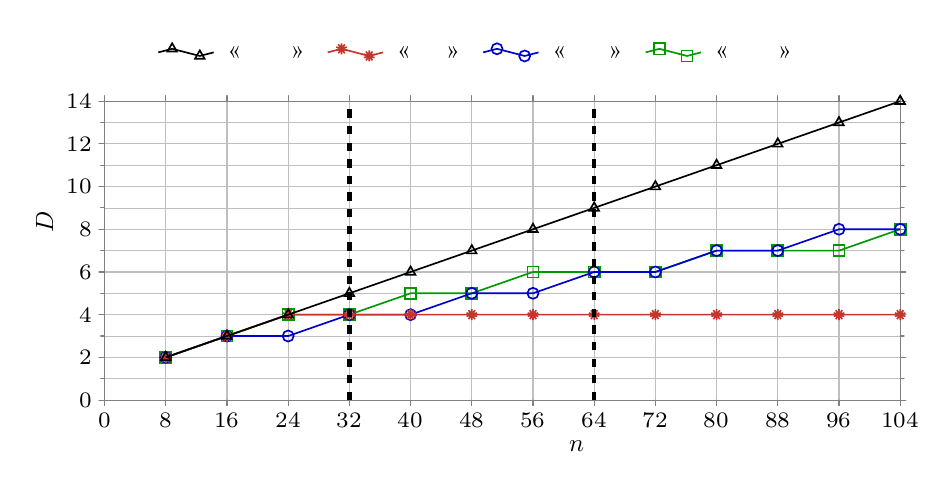
\begin{tikzpicture}
						\datavisualization [
							scientific axes,
							all axes = {
								grid,
								include value = 0,
							},
							x axis = {
								attribute = x,
								length = 10\gridunitwidth,
								ticks = {
									step = 8,
								},
								label = {Кількість процесорів~$n$},
							},
							y axis = {
								attribute = y,
								length = 9\baselineskip,
								ticks = {
									step = 2,
									minor steps between steps = 1,
								},
								label = {Діаметр~$D$},
							},
							legend = {%
								above,
							},
							style sheet = strong colors,
							visualize as line/.list = {topology-line, topology-star, topology-ring, topology-grid},
							%
							topology-line = {
								style = {
									mark = triangle,
								},
								label in legend = {%
									text = {«Лінійка»},
								},
							},
							%
							topology-star = {
								style = {
									mark = 10-pointed star,
								},
								label in legend = {%
									text = {«Зірка»},
								},
							},
							%
							topology-ring = {
								style = {
									mark = o,
								},
								label in legend = {%
									text = {«Кільце»},
								},
							},
							%
							topology-grid = {
								style = {
									mark = square,
								},
								label in legend = {%
									text = {«Решітка»},
								},
							},
							%
						]
							data [set = topology-line] {
								x, y
								8, 2
								16, 3
								24, 4
								32, 5
								40, 6
								48, 7
								56, 8
								64, 9
								72, 10
								80, 11
								88, 12
								96, 13
								104, 14
							}

							data [set = topology-star] {
								x, y
								8, 2
								16, 3
								24, 4
								32, 4
								40, 4
								48, 4
								56, 4
								64, 4
								72, 4
								80, 4
								88, 4
								96, 4
								104, 4
							}

							data [set = topology-ring] {
								x, y
								8, 2
								16, 3
								24, 3
								32, 4
								40, 4
								48, 5
								56, 5
								64, 6
								72, 6
								80, 7
								88, 7
								96, 8
								104, 8
							}

							data [set = topology-grid] {
								x, y
								8, 2
								16, 3
								24, 4
								32, 4
								40, 5
								48, 5
								56, 6
								64, 6
								72, 6
								80, 7
								88, 7
								96, 7
								104, 8
							}

							info {
								\draw [dashed, ultra thick] (visualization cs: x=32, y=0) -- (visualization cs: x=32, y=14);
								\draw [dashed, ultra thick] (visualization cs: x=64, y=0) -- (visualization cs: x=64, y=14);
							};
					\end{tikzpicture}
					\caption{Графік залежності діаметра~$D$ для топологій «Лінійка», «Зірка», «Кільце» і~«Решітка»}
					\label{fig:plot-comparison-diameter}
				\end{figure}

				\begin{figure}[!htbp]
					\centering
					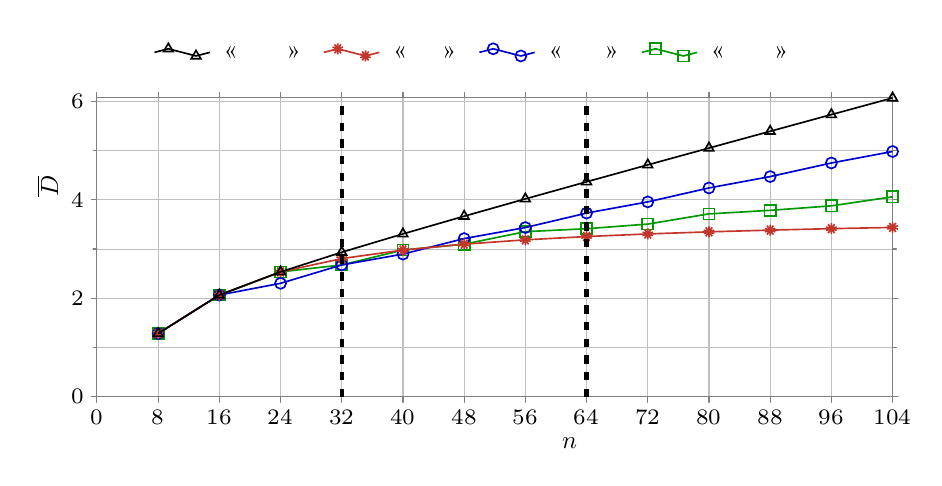
\begin{tikzpicture}
						\datavisualization [
							scientific axes,
							all axes = {
								grid,
								include value = 0,
							},
							x axis = {
								attribute = x,
								length = 10\gridunitwidth,
								ticks = {
									step = 8,
								},
								label = {Кількість процесорів~$n$},
							},
							y axis = {
								attribute = y,
								length = 9\baselineskip,
								ticks = {
									step = 2,
									minor steps between steps = 1,
								},
								label = {Середній діаметр~$\overline{D}$},
							},
							legend = {%
								above,
							},
							style sheet = strong colors,
							visualize as line/.list = {topology-line, topology-star, topology-ring, topology-grid},
							%
							topology-line = {
								style = {
									mark = triangle,
								},
								label in legend = {%
									text = {«Лінійка»},
								},
							},
							%
							topology-star = {
								style = {
									mark = 10-pointed star,
								},
								label in legend = {%
									text = {«Зірка»},
								},
							},
							%
							topology-ring = {
								style = {
									mark = o,
								},
								label in legend = {%
									text = {«Кільце»},
								},
							},
							%
							topology-grid = {
								style = {
									mark = square,
								},
								label in legend = {%
									text = {«Решітка»},
								},
							},
							%
						]
							data [set = topology-line] {
								x, y
								8, 1.28571428571428
								16, 2.06666666666666
								24, 2.53623188405797
								32, 2.93548387096774
								40, 3.3076923076923
								48, 3.66666666666666
								56, 4.01818181818181
								64, 4.36507936507936
								72, 4.70892018779342
								80, 5.0506329113924
								88, 5.39080459770114
								96, 5.7298245614035
								104, 6.06796116504854
							}

							data [set = topology-star] {
								x, y
								8, 1.28571428571428
								16, 2.06666666666666
								24, 2.53623188405797
								32, 2.80645161290322
								40, 2.97948717948717
								48, 3.09929078014184
								56, 3.18701298701298
								64, 3.25396825396825
								72, 3.30672926447574
								80, 3.34936708860759
								88, 3.38453500522466
								96, 3.41403508771929
								104, 3.43913368185212
							}

							data [set = topology-ring] {
								x, y
								8, 1.28571428571428
								16, 2.06666666666666
								24, 2.30434782608695
								32, 2.6774193548387
								40, 2.89743589743589
								48, 3.2127659574468
								56, 3.43636363636363
								64, 3.73015873015873
								72, 3.95774647887323
								80, 4.24050632911392
								88, 4.47126436781609
								96, 4.74736842105263
								104, 4.98058252427184
							}

							data [set = topology-grid] {
								x, y
								8, 1.28571428571428
								16, 2.06666666666666
								24, 2.53623188405797
								32, 2.6774193548387
								40, 2.97948717948717
								48, 3.09929078014184
								56, 3.35324675324675
								64, 3.41269841269841
								72, 3.50704225352112
								80, 3.71392405063291
								88, 3.78578892371995
								96, 3.87719298245614
								104, 4.06049290515309
							}

							info {
								\draw [dashed, ultra thick] (visualization cs: x=32, y=0) -- (visualization cs: x=32, y=6);
								\draw [dashed, ultra thick] (visualization cs: x=64, y=0) -- (visualization cs: x=64, y=6);
							};
					\end{tikzpicture}
					\caption{Графік залежності середнього діаметра~$\overline{D}$ для топологій «Лінійка», «Зірка», «Кільце» і~«Решітка»}
					\label{fig:plot-comparison-avg-diameter}
				\end{figure}

				\begin{figure}[!htbp]
					\centering
					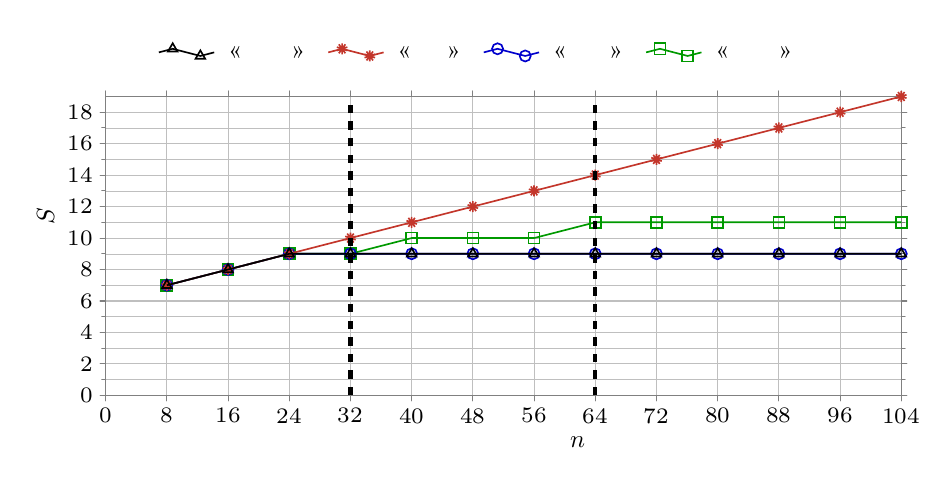
\begin{tikzpicture}
						\datavisualization [
							scientific axes,
							all axes = {
								grid,
								include value = 0,
							},
							x axis = {
								attribute = x,
								length = 10\gridunitwidth,
								ticks = {
									step = 8,
								},
								label = {Кількість процесорів~$n$},
							},
							y axis = {
								attribute = y,
								length = 9\baselineskip,
								ticks = {
									step = 2,
									minor steps between steps = 1,
								},
								label = {Ступень~$S$},
							},
							legend = {%
								above,
							},
							style sheet = strong colors,
							visualize as line/.list = {topology-line, topology-star, topology-ring, topology-grid},
							%
							topology-line = {
								style = {
									mark = triangle,
								},
								label in legend = {%
									text = {«Лінійка»},
								},
							},
							%
							topology-star = {
								style = {
									mark = 10-pointed star,
								},
								label in legend = {%
									text = {«Зірка»},
								},
							},
							%
							topology-ring = {
								style = {
									mark = o,
								},
								label in legend = {%
									text = {«Кільце»},
								},
							},
							%
							topology-grid = {
								style = {
									mark = square,
								},
								label in legend = {%
									text = {«Решітка»},
								},
							},
							%
						]
							data [set = topology-line] {
								x, y
								008, 7
								016, 8
								024, 9
								032, 9
								040, 9
								048, 9
								056, 9
								064, 9
								072, 9
								080, 9
								088, 9
								096, 9
								104, 9
							}

							data [set = topology-star] {
								x, y
								008, 07
								016, 08
								024, 09
								032, 10
								040, 11
								048, 12
								056, 13
								064, 14
								072, 15
								080, 16
								088, 17
								096, 18
								104, 19
							}

							data [set = topology-ring] {
								x, y
								008, 7
								016, 8
								024, 9
								032, 9
								040, 9
								048, 9
								056, 9
								064, 9
								072, 9
								080, 9
								088, 9
								096, 9
								104, 9
							}

							data [set = topology-grid] {
								x, y
								008, 07
								016, 08
								024, 09
								032, 09
								040, 10
								048, 10
								056, 10
								064, 11
								072, 11
								080, 11
								088, 11
								096, 11
								104, 11
							}

							info {
								\draw [dashed, ultra thick] (visualization cs: x=32, y=0) -- (visualization cs: x=32, y=19);
								\draw [dashed, ultra thick] (visualization cs: x=64, y=0) -- (visualization cs: x=64, y=19);
							};
					\end{tikzpicture}
					\caption{Графік залежності ступеня~$S$ для топологій «Лінійка», «Зірка», «Кільце» і~«Решітка»}
					\label{fig:plot-comparison-degree}
				\end{figure}

				\begin{figure}[!htbp]
					\centering
					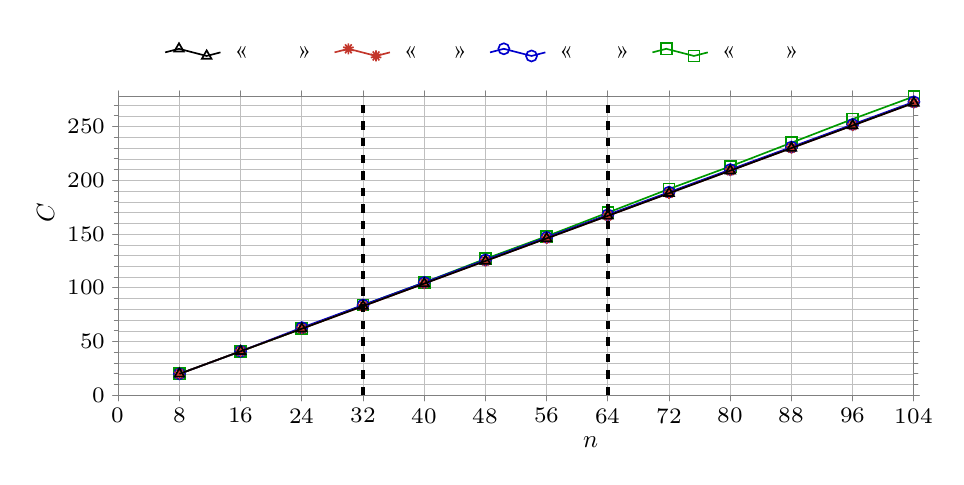
\begin{tikzpicture}
						\datavisualization [
							scientific axes,
							all axes = {
								grid,
								include value = 0,
							},
							x axis = {
								attribute = x,
								length = 10\gridunitwidth,
								ticks = {
									step = 8,
								},
								label = {Кількість процесорів~$n$},
							},
							y axis = {
								attribute = y,
								length = 9\baselineskip,
								ticks = {
									step = 50,
									minor steps between steps = 4,
								},
								label = {Вартість~$C$},
							},
							legend = {%
								above,
							},
							style sheet = strong colors,
							visualize as line/.list = {topology-line, topology-star, topology-ring, topology-grid},
							%
							topology-line = {
								style = {
									mark = triangle,
								},
								label in legend = {%
									text = {«Лінійка»},
								},
							},
							%
							topology-star = {
								style = {
									mark = 10-pointed star,
								},
								label in legend = {%
									text = {«Зірка»},
								},
							},
							%
							topology-ring = {
								style = {
									mark = o,
								},
								label in legend = {%
									text = {«Кільце»},
								},
							},
							%
							topology-grid = {
								style = {
									mark = square,
								},
								label in legend = {%
									text = {«Решітка»},
								},
							},
							%
						]
							data [set = topology-line] {
								x, y
								008, 020
								016, 041
								024, 062
								032, 083
								040, 104
								048, 125
								056, 146
								064, 167
								072, 188
								080, 209
								088, 230
								096, 251
								104, 272
							}

							data [set = topology-star] {
								x, y
								008, 020
								016, 041
								024, 062
								032, 083
								040, 104
								048, 125
								056, 146
								064, 167
								072, 188
								080, 209
								088, 230
								096, 251
								104, 272
							}

							data [set = topology-ring] {
								x, y
								008, 020
								016, 041
								024, 063
								032, 084
								040, 105
								048, 126
								056, 147
								064, 168
								072, 189
								080, 210
								088, 231
								096, 252
								104, 273
							}

							data [set = topology-grid] {
								x, y
								008, 020
								016, 041
								024, 062
								032, 084
								040, 105
								048, 127
								056, 148
								064, 170
								072, 192
								080, 213
								088, 235
								096, 257
								104, 278
							}

							info {
								\draw [dashed, ultra thick] (visualization cs: x=32, y=0) -- (visualization cs: x=32, y=278);
								\draw [dashed, ultra thick] (visualization cs: x=64, y=0) -- (visualization cs: x=64, y=278);
							};
					\end{tikzpicture}
					\caption{Графік залежності вартості~$C$ для топологій «Лінійка», «Зірка», «Кільце» і~«Решітка»}
					\label{fig:plot-comparison-cost}
				\end{figure}

				\begin{figure}[!htbp]
					\centering
					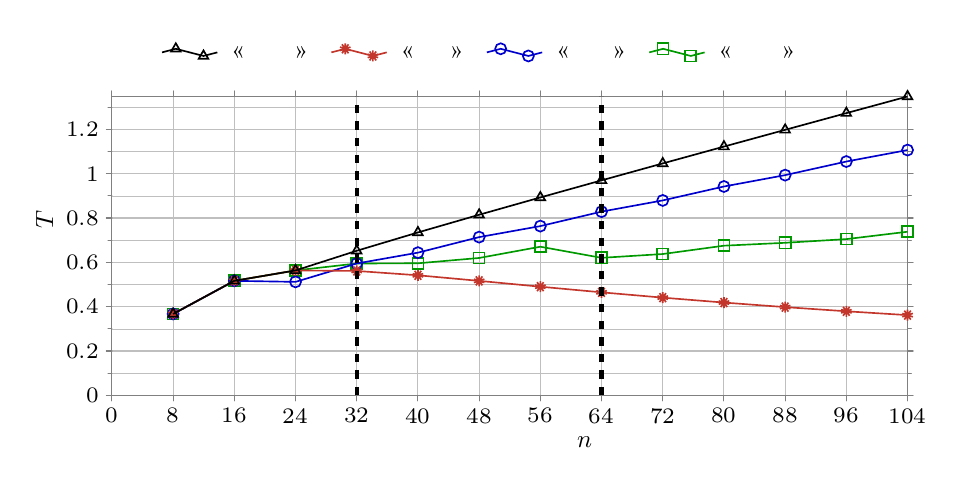
\begin{tikzpicture}
						\datavisualization [
							scientific axes,
							all axes = {
								grid,
								include value = 0,
							},
							x axis = {
								attribute = x,
								length = 10\gridunitwidth,
								ticks = {
									step = 8,
								},
								label = {Кількість процесорів~$n$},
							},
							y axis = {
								attribute = y,
								length = 9\baselineskip,
								ticks = {
									step = 0.2,
									minor steps between steps = 1,
								},
								label = {Трафік~$T$},
							},
							legend = {%
								above,
							},
							style sheet = strong colors,
							visualize as line/.list = {topology-line, topology-star, topology-ring, topology-grid},
							%
							topology-line = {
								style = {
									mark = triangle,
								},
								label in legend = {%
									text = {«Лінійка»},
								},
							},
							%
							topology-star = {
								style = {
									mark = 10-pointed star,
								},
								label in legend = {%
									text = {«Зірка»},
								},
							},
							%
							topology-ring = {
								style = {
									mark = o,
								},
								label in legend = {%
									text = {«Кільце»},
								},
							},
							%
							topology-grid = {
								style = {
									mark = square,
								},
								label in legend = {%
									text = {«Решітка»},
								},
							},
							%
						]
							data [set = topology-line] {
								x, y
								008, 0.36734693877551
								016, 0.516666666666666
								024, 0.563607085346215
								032, 0.652329749103942
								040, 0.735042735042735
								048, 0.814814814814814
								056, 0.892929292929293
								064, 0.970017636684303
								072, 1.04642670839853
								080, 1.12236286919831
								088, 1.19795657726692
								096, 1.27329434697855
								104, 1.34843581445523
							}

							data [set = topology-star] {
								x, y
								008, 0.36734693877551
								016, 0.516666666666666
								024, 0.563607085346215
								032, 0.561290322580645
								040, 0.541724941724941
								048, 0.516548463356974
								056, 0.49030969030969
								064, 0.46485260770975
								072, 0.440897235263432
								080, 0.418670886075949
								088, 0.39818058884996
								096, 0.37933723196881
								104, 0.362014071773908
							}

							data [set = topology-ring] {
								x, y
								008, 0.36734693877551
								016, 0.516666666666666
								024, 0.51207729468599
								032, 0.594982078853046
								040, 0.643874643874643
								048, 0.713947990543735
								056, 0.763636363636363
								064, 0.828924162257495
								072, 0.879499217527386
								080, 0.942334739803094
								088, 0.993614303959131
								096, 1.05497076023391
								104, 1.10679611650485
							}

							data [set = topology-grid] {
								x, y
								008, 0.36734693877551
								016, 0.516666666666666
								024, 0.563607085346215
								032, 0.594982078853046
								040, 0.595897435897435
								048, 0.619858156028368
								056, 0.67064935064935
								064, 0.62049062049062
								072, 0.63764404609475
								080, 0.675258918296893
								088, 0.688325258858174
								096, 0.704944178628389
								104, 0.738271437300563
							}

							info {
								\draw [dashed, ultra thick] (visualization cs: x=32, y=0) -- (visualization cs: x=32, y=1.34843581445523);
								\draw [dashed, ultra thick] (visualization cs: x=64, y=0) -- (visualization cs: x=64, y=1.34843581445523);
							};
					\end{tikzpicture}
					\caption{Графік залежності трафіка~$T$ для топологій «Лінійка», «Зірка», «Кільце» і~«Решітка»}
					\label{fig:plot-comparison-traffic}
				\end{figure}

		\subsection{Порівняльний аналіз}
			Побудувавши графіки залежностей топологічних характеристик від кількості процесорів для кожної топології, порівняємо значення цих характеристик. Для цього розділимо графіки на~3~зони. Границі зон визначаються там, де~є~найбільше точок перетину графіків залежності діаметру~$D$ від кількості процесорів. Тому отримаємо зони з~такими границями:
			\begin{enumerate}
				\item Від 1 до~32 процесорів.
				\item Від 33 до~64 процесорів.
				\item Від 65 до~104 процесорів.
			\end{enumerate}
			Обчислимо середні значення топологічних характеристик для кожної із~зон і~занесемо отримані результати у~таблиці, відповідні кожній зоні~(зона~1~— табл.~\ref{tab:table-comparison-zone-01}, зона~1~— табл.~\ref{tab:table-comparison-zone-02}, зона~1~— табл.~\ref{tab:table-comparison-zone-03}).

			\begin{table}[!htbp]
				\centering
				\caption{Середні значення топологічних характеристик топологій «Лінійка», «Зірка», «Кільце» і~«Решітка» для зони~1~(кількість процесорів~$n$ від~1 до~32)}
				\label{tab:table-comparison-zone-01}
				\begin{tabular}{
						v{2\gridunitwidth - 2\tabcolsep}
						S[%
							table-column-width={2\gridunitwidth - 2\tabcolsep},
							table-format=1.2,
							table-auto-round,
							table-alignment=right,
						]
						S[%
							table-column-width={2\gridunitwidth - 2\tabcolsep},
							table-format=1.3,
							table-auto-round,
							table-alignment=right,
						]
						S[%
							table-column-width={2\gridunitwidth - 2\tabcolsep},
							table-format=2.2,
							table-auto-round,
							table-alignment=right,
						]
						S[%
							table-column-width={2\gridunitwidth - 2\tabcolsep},
							table-format=4.2,
							table-auto-round,
							table-alignment=right,
						]
						S[%
							table-column-width={2\gridunitwidth - 2\tabcolsep},
							table-format=1.3,
							table-auto-round,
							table-alignment=right,
						]
				}
					\toprule
						{Топологія} &
						{Діаметр~$D$} &
						{Сер. діам.~$\overline{D}$} &
						{Степінь~$S$} &
						{Вартість~$C$} &
						{Трафік~$T$} \\
					\midrule
						Лінійка & 3,5 & 2,20602417685166 & 8,25 & 51,5 & 0,524987609973083 \\
						Зірка & 3,25 & 2,17376611233553 & 8,5 & 51,5 & 0,502227753342259 \\
						Кільце & 3 & 2,08353703332665 & 8,25 & 52 & 0,497768244745303 \\
						Решітка & 3,25 & 2,1415080478194 & 8,6 & 51,75 & 0,510650692410359 \\
					\bottomrule
				\end{tabular}
			\end{table}

			\begin{table}[!htbp]
				\centering
				\caption{Середні значення топологічних характеристик топологій «Лінійка», «Зірка», «Кільце» і~«Решітка» для зони~2~(кількість процесорів~$n$ від~33 до~64)}
				\label{tab:table-comparison-zone-02}
				\begin{tabular}{
						v{2\gridunitwidth - 2\tabcolsep}
						S[%
							table-column-width={2\gridunitwidth - 2\tabcolsep},
							table-format=1.2,
							table-auto-round,
							table-alignment=right,
						]
						S[%
							table-column-width={2\gridunitwidth - 2\tabcolsep},
							table-format=1.3,
							table-auto-round,
							table-alignment=right,
						]
						S[%
							table-column-width={2\gridunitwidth - 2\tabcolsep},
							table-format=2.2,
							table-auto-round,
							table-alignment=right,
						]
						S[%
							table-column-width={2\gridunitwidth - 2\tabcolsep},
							table-format=4.2,
							table-auto-round,
							table-alignment=right,
						]
						S[%
							table-column-width={2\gridunitwidth - 2\tabcolsep},
							table-format=1.3,
							table-auto-round,
							table-alignment=right,
						]
				}
					\toprule
						{Топологія} &
						{Діаметр~$D$} &
						{Сер. діам.~$\overline{D}$} &
						{Степінь~$S$} &
						{Вартість~$C$} &
						{Трафік~$T$} \\
					\midrule
						Лінійка & 7,5 & 3,83940503940503 & 9 & 135,5 & 0,853201119867786 \\
						Зірка & 4 & 3,12993980015256 & 12,5 & 135,5 & 0,503358925775339 \\
						Кільце & 5 & 3,31918105535126 & 9 & 136,5 & 0,737595790078059 \\
						Решітка & 5,5 & 3,21118078139354 & 10,25 & 137,5 & 0,626723890766443 \\
					\bottomrule
				\end{tabular}
			\end{table}

			\begin{table}[!htbp]
				\centering
				\caption{Середні значення топологічних характеристик топологій «Лінійка», «Зірка», «Кільце» і~«Решітка» для зони~3~(кількість процесорів~$n$ від~65 до~104)}
				\label{tab:table-comparison-zone-03}
				\begin{tabular}{
						v{2\gridunitwidth - 2\tabcolsep}
						S[%
							table-column-width={2\gridunitwidth - 2\tabcolsep},
							table-format=1.2,
							table-auto-round,
							table-alignment=right,
						]
						S[%
							table-column-width={2\gridunitwidth - 2\tabcolsep},
							table-format=1.3,
							table-auto-round,
							table-alignment=right,
						]
						S[%
							table-column-width={2\gridunitwidth - 2\tabcolsep},
							table-format=2.2,
							table-auto-round,
							table-alignment=right,
						]
						S[%
							table-column-width={2\gridunitwidth - 2\tabcolsep},
							table-format=4.2,
							table-auto-round,
							table-alignment=right,
						]
						S[%
							table-column-width={2\gridunitwidth - 2\tabcolsep},
							table-format=1.3,
							table-auto-round,
							table-alignment=right,
						]
				}
					\toprule
						{Топологія} &
						{Діаметр~$D$} &
						{Сер. діам.~$\overline{D}$} &
						{Степінь~$S$} &
						{Вартість~$C$} &
						{Трафік~$T$} \\
					\midrule
						Лінійка & 12 & 5,3896286846678 & 9 & 230 & 1,19769526325951 \\
						Зірка & 4 & 3,37876002557588 & 17 & 230 & 0,399820002786412 \\
						Кільце & 7,2 & 4,47949362422554 & 9 & 231 & 0,995443027605674 \\
						Решітка & 7 & 3,78888822309664 & 11 & 235 & 0,688888767835754 \\
					\bottomrule
				\end{tabular}
			\end{table}

			Оцінимо отримані середні значення топологічної характеристики за~шкалою від~1 до~5~балів. Пам'ятаємо, що~для діаметру~$D$, середнього діаметру~$\overline{D}$, ступеня~$S$ і~вартості~$C$ оптимальним є~найменше значення. Оптимальне значення трафіку~$T = 1$.
			
			Для оцінки характеристик використовуємо таку послідовність дій:
			\begin{enumerate}
				\item Знаходимо мінімальне і~максимальне значення даної характеристики в~усіх зонах: $c_{\text{min}}$ і~$c_{\text{max}}$.
				\item Знаходимо крок інтервалу оцінки~$s$: різницю максимального і~мінімального значення: $s = c_{\text{max}} - c_{\text{min}}$.
				\item Знаходимо інтервали для відповідних оцінок. Якщо оптимальне значення характеристики найменше, ліва границя інтервалу для найвищої оцінки~$b_{l}$~— мінімальне значення характеристики в~усіх зонах: $b_{l} = c_{\text{min}}$. Тоді права границя~$b_{r}$ буде сумою лівої границі і~кроку інтервалу оцінки: $b_{l} + s$. Наприклад, якщо оптимальним є~найменше значення, то~для найвищої оцінки~«5» отримуємо такий інтервал: $i_{5} = \left[c_{\text{min}}; c_{\text{min}} + s\right)$. Повторюємо для всіх оцінок.
				\item Визначивши інтервали, в~залежності від того, в~який з~інтервалів попадає значення характеристики, присвоюємо йому відповідну оцінку і~записуємо~її~в~таблицю.
			\end{enumerate}
			%Оцінюємо значення характеристик по~всім зонам, знайшовши мінімальне та~максимальне значення характеристики, далі знаходимо їх~різницю, ділимо на~кількість оцінок і~отримаємо інтервали, що~відповідають певній оцінці.
			Результати оцінки заносимо у~відповідні зонам таблиці~(зона~1~— табл.~\ref{tab:table-comparison-zone-01-marks}, зона~3~— табл.~\ref{tab:table-comparison-zone-02-marks}, зона~3~— табл.~\ref{tab:table-comparison-zone-03-marks}).

			\begin{table}[!htbp]
				\centering
				\caption{Оцінки значень топологічних характеристик топологій «Лінійка», «Зірка», «Кільце» і~«Решітка» для зони~1~(кількість процесорів~$n$ від~1 до~32)}
				\label{tab:table-comparison-zone-01-marks}
				\begin{tabular}{
						v{2\gridunitwidth - 2\tabcolsep}
						*{5}{n{2\gridunitwidth - 2\tabcolsep}}
				}
					\toprule
						{Топологія} &
						{Діаметр~$D$} &
						{Сер. діаметр~$\overline{D}$} &
						{Степінь~$S$} &
						{Вартість~$C$} &
						{Трафік~$T$} \\
					\midrule
						Лінійка & 5 & 5 & 5 & 5 & 1 \\
						Зірка & 5 & 5 & 5 & 5 & 1 \\
						Кільце & 5 & 5 & 5 & 5 & 1 \\
						Решітка & 5 & 5 & 5 & 5 & 1 \\
					\bottomrule
				\end{tabular}
			\end{table}

			\begin{table}[!htbp]
				\centering
				\caption{Оцінки значень топологічних характеристик топологій «Лінійка», «Зірка», «Кільце» і~«Решітка» для зони~2~(кількість процесорів~$n$ від~33 до~64)}
				\label{tab:table-comparison-zone-02-marks}
				\begin{tabular}{
						v{2\gridunitwidth - 2\tabcolsep}
						*{5}{n{2\gridunitwidth - 2\tabcolsep}}
				}
					\toprule
						{Топологія} &
						{Діаметр~$D$} &
						{Сер. діаметр~$\overline{D}$} &
						{Степінь~$S$} &
						{Вартість~$C$} &
						{Трафік~$T$} \\
					\midrule
						Лінійка & 3 & 3 & 5 & 3 & 4 \\
						Зірка & 5 & 4 & 3 & 3 & 1 \\
						Кільце & 4 & 4 & 5 & 3 & 3 \\
						Решітка & 4 & 4 & 4 & 3 & 2 \\
					\bottomrule
				\end{tabular}
			\end{table}

			\begin{table}[!htbp]
				\centering
				\caption{Оцінки значень топологічних характеристик топологій «Лінійка», «Зірка», «Кільце» і~«Решітка» для зони~3~(кількість процесорів~$n$ від~65 до~104)}
				\label{tab:table-comparison-zone-03-marks}
				\begin{tabular}{
						v{2\gridunitwidth - 2\tabcolsep}
						*{5}{n{2\gridunitwidth - 2\tabcolsep}}
				}
					\toprule
						{Топологія} &
						{Діаметр~$D$} &
						{Сер. діаметр~$\overline{D}$} &
						{Степінь~$S$} &
						{Вартість~$C$} &
						{Трафік~$T$} \\
					\midrule
						Лінійка & 1 & 1 & 5 & 1 & 4 \\
						Зірка & 5 & 3 & 1 & 1 & 1 \\
						Кільце & 3 & 2 & 5 & 1 & 5 \\
						Решітка & 3 & 3 & 4 & 1 & 3 \\
					\bottomrule
				\end{tabular}
			\end{table}

			За~побудованими таблицями оцінок для кожної з~зон складаємо таблицю сумарних оцінок за~зонами та~підсумкових оцінок для топології~(табл.~\ref{tab:table-comparison-total}).

			\begin{table}[!htbp]
				\centering
				\caption{Сумарні оцінки значень топологічних характеристик топологій «Лінійка», «Зірка», «Кільце» і~«Решітка»}
				\label{tab:table-comparison-total}
				\begin{tabular}{
						v{2.25\gridunitwidth - 2\tabcolsep}
						n{2.50\gridunitwidth - 2\tabcolsep}
						n{2.50\gridunitwidth - 2\tabcolsep}
						n{2.50\gridunitwidth - 2\tabcolsep}
						n{2.25\gridunitwidth - 2\tabcolsep}
				}
					\toprule
						& \multicolumn{3}{c}{Оцінка для різних зон} & \\
						\cmidrule(lr){2-4}
						{Топологія} &
						Зона~1: $n \in [1; 32]$ &
						Зона~2: $n \in [33; 64]$ &
						Зона~3: $n \in [65; 104]$ &
						Сумарна оцінка\\
					\midrule
						Лінійка & 21 & 18 & 12 & 51 \\
						Зірка & 21 & 16 & 11 & 48 \\
						Кільце & 21 & 19 & 16 & 56 \\
						Решітка & 21 & 17 & 14 & 52 \\
					\bottomrule
				\end{tabular}
			\end{table}

		Отже, отримали порівняльну оцінку топологій «Лінійка», «Зірка», «Кільце» і~«Решітка» для масштабування паралельної системи на~основі заданого кластера.

	\section{Висновок}
		Виконуючи даний курсовий проект, були досліджені основні топологічні характеристики паралельних обчислювальних систем з~масивно-паралельними архітектурами зі~статичними зв'язками між процесорами. Характеристики розглядались на~прикладі систем, організованих із~заданих обчислювальних кластерів, з~різними топологіями: «Лінійка», «Зірка», «Кільце», «Решітка».

		Дослідження показало, що~при невеликій кількості процесорів (від~1 до~32) досліджувані топології поводяться майже однаково: різниця у~топологічних характеристиках незначна. Також виявлено, що~вартість для різних топологій незмінно зростає за~лінійним законом, так як~нові кластери лише додаються, і~тому кількість зв'язків у~системі пропорційно збільшується.

		Зі~збільшенням кількості процесорів у~системі топології поводять себе по-різному. Наприклад, у~топології «Лінійка» лінійно зростають діаметр, середній діаметр і~трафік, тобто значення цих~характеристик погіршуються і~швидко виходять за~межі бажаних.

		При масштабуванні топології «Зірка» діаметр перестає зростати вже на~4~кроці, при 32~процесорах. Водночас стрімко зростає степінь системи. Фактично, топологія «Зірка» позбавляється лінійного зростання діаметра і~середнього діаметра ціною такого ж~стрімкого зростання степеня. На~відміну від «Лінійки», де~зі~збільшенням кількості процесорів значення трафіка лінійно зростає, в~топології «Зірка» його значення так само лінійно спадає, тим самим відхиляючись від оптимального значення~$T = 1$. Тому з~точки зору поведінки діаметра, середнього діаметра і~трафіка топології «Лінійка» і~«Зірка» є~протилежними.

		Плавне зростання діаметра, середнього діаметра і~степеня на~прикладі даного кластера спостерігається при масштабуванні топологій~«Кільце» і~«Решітка», однак, від середини масштабування (кількість процесорів~$n > 32$) і~аж~до~кінцевого кроку топологія «Кільце» мала кращі значення вищезгаданих параметрів, ніж «Решітка»: значення трафіка наближалась до~оптимального, поки відхилення від оптимального значення для «Решітки» було вдвічі більшим. Тому можна сказати, що~для масштабування даного конкретного кластеру до~першого кроку, на~якому кількість процесорів перевищить~100, є~топологія «Кільце».

		Загалом, судячи з~результатів дослідження, проведеного в~рамках даного курсового проекту, зрозуміло, що~системи «Лінійка» і~«Зірка» недоцільні для паралельних систем з~масивно-паралельними архітектурами великих масштабів, в~той час як~«Кільце» і~«Решітка» будуть оптимальними для таких задач, адже їх~характеристики значно повільніше відхиляються від відповідних оптимальних значень. Зі~збільшенням кількості процесорів найкращі характеристики матиме «Решітка», оскільки графіки показують, що~значення її~топологічних характеристик ростуть повільніше, а~отже й~менше відхиляються від бажаних, ніж аналогічні значення для топології «Кільце».

		\section{Список використаної літератури}
			\begin{manualbib}[widest=10]
				\item Богданов~А.\,В., Корхов~В.\,В., Мареев~В.\,В., Станкова~Е.\,Н. Архитектуры и~топологии многопроцессорныхх вычислительных систем. Интернет-университет информационных технологий — ИНТУИТ.ру, 2004.
				\item Бройдо~В. Вычислительные системы, сети и~телекоммуникации. — СПб.: Питер, 2002. — 688 с.
				\item Головкин~Б.\,А.~Вычислительные системи с~большим числом процессоров. — М.: Радио и~связь, 1995. — 320 с.
				\item Коуги~П.\,М. Архитектура конвейерных ЭОМ: Пер. с~англ. — М.: Радио и~связь, 1985.
				\item Обчислювальні системи: Лабораторні роботи 1–4 / Уклад.: І.\,А.~Жуков, Є.\,В.~Красовська. — К~.: НАУ, 2003. — 34 с.
				\item Обчислювальні системи: Лабораторні роботи 5, 6 / Уклад.: І.\,А.~Жуков, Є.\,В.~Красовська, О.\,В.~Русанова. — К~.: НАУ, 2005. — 16 с.
				\item Обчислювальні системи: Лабораторні роботи 7, 8 / Уклад.: І.\,А.~Жуков, Є.\,В.~Красовська, О.\,В.~Русанова. — К~.: НАУ, 2007. — 28 с.
				\item Основы теории вычислительных систем: Учебное пособие / Под ред. С.\,А.~Майорова. — М.: Высш. шк., 1978. — 260 с.
				\item Самофалов~К.\,Г., Луцкий~Г.\,М. Основы теории многоуровневых конвейерных вычислительных систем. — М.: Радио и~связь, 1989. — 272 с.
				\item Цилькер~Б.\,Я., Орлов~С.\,А. Организация ЭВМ и~систем: Учебник для вузов. — СПб.: Питер, 2006. — 668 с. 
			\end{manualbib}

\end{document}

